\documentclass[a4paper]{article}

\usepackage{ReportTemplate}
\usepackage{setspace}
\usepackage{amsmath}
\usepackage[hidelinks]{hyperref}

\title{随机森林的实现以及节点分类函数探究
}
\name{谢炜基}
\studentid{521030910421}

\begin{document}

\maketitle



\section{从0实现随机森林分类器}

\subsection{实现细节}
\subsubsection{工作原理}
随机森林包含\texttt{n\_estimators}个基决策树, 每个决策树都是二叉树, 由许多自相似的节点构成. 

在训练随机森林分类器时, 先依据预定的方式(由参数\texttt{bootstrap},\texttt{max\_samples}确定)获取用于训练每个基决策树的样本, 再从每个基决策树的根节点出发递归地训练决策树.

在训练每个节点时, 给定训练样本, 先随机选取\texttt{m} $\leq$\texttt{ max\_features}个备选特征, 依据预定的判断准则来分别计算选取每个特征作为该节点的分裂特征能带来的信息增益. 在确定带来最大信息增益的特征后, 寻找该特征中能带来最大分裂增益的特征值. 依据这个分裂特征和分裂值, 将训练样本分为两类, 分别用于训练该节点的两个子节点. 

分裂增益的计算方法是$ g(Y)-\frac{N_l}{N}g(Y_l)-\frac{N_r}{N}g(Y_r) $, 其中$g$是判别准则, $Y$是该节点的训练样本的标签,  $Y_l,Y_r$分别是分裂至左子节点和右子节点的样本标签, $N,N_l,N_r$分别是该节点, 左子节点, 右子节点的训练样本个数.分裂停止的判别依据是下述的参数: \texttt{max\_depth}, \texttt{min\_samples\_split}, \texttt{min\_samples\_leaf},  \texttt{min\_impurity\_decrease}.

在判定某个节点应当成为叶节点而不应当分裂后, 该节点的预测值根据它的训练样本的标签投票确定, 有软预测和硬预测两种类型.

在分类器进行预测时, 待分类样本进入每个基决策树, 依据各个节点的分裂特征和分裂值将样本传入子节点, 将它最终达到的叶节点的预测值作为该基决策树的预测值. 得到所有基决策树的预测值后, 采用平均投票的方式获得该样本的最终类别预测.

\subsubsection{模型参数}
我们参考\texttt{sklearn}中的随机森林API\cite{sklearn}, 使用\textbf{python}实现了包含以下参数的随机森林分类器.
\begin{itemize}
    \item \texttt{n\_estimators}: 随机森林中基决策树的个数. 默认为10. 
    \item \texttt{n\_jobs}: 并行训练基决策树时的并行任务数. 在通常情况下也即程序可同时利用的最大CPU核数. 默认为4. 
    \item \texttt{criterion}: 评价节点分裂的质量的方法.可选\texttt{'gini'}/\texttt{'entropy'}. 默认为\texttt{'gini'}.
    \item \texttt{soft\_pred}: 叶节点的预测是否为概率值. 若为False, 表示叶节点的预测为该节点中包含最多样本的类别. 若为True, 表示叶节点的预测为该节点包含的样本中各个类别的出现频率. 默认为False. 
    \item \texttt{max\_depth}: 每个基决策树的最大深度. 若为None, 表示不限制基树的深度. 默认为None.
    \item \texttt{min\_samples\_split}: 继续分裂一个节点所需的最小样本数. 若一个节点的样本数低于这个值, 则不再分裂这个节点, 这个节点成为叶节点. 默认为2.
    \item \texttt{min\_samples\_leaf}: 叶节点包含的最小样本数. 若分裂某个节点时将会产生的叶节点所含样本数低于这个值, 则不分裂这个节点. 默认为1.
    \item \texttt{max\_features}: 在决定每个叶节点的分裂特征和分裂值时, 候选的特征数量的最大值. 这个参数的候选值是$(0,1]$的浮点数, 表示候选特征最大值占总特征数的比例. 默认为None, 表示候选特征最大值是总特征数开根号.
    \item \texttt{min\_impurity\_decrease}: 分裂节点时要求的最小不纯度下降值. 若不纯度下降值低于这个值, 则不分裂该节点. 默认为0.
    \item \texttt{bootstrap}: 训练每个基树的样本是否采用bootstrap方法选取. 默认为True.
    \item \texttt{max\_samples}: 训练每个基树时使用的样本数. 参数的取值为$(0,1]$的浮点数, 表示它占总样本数的比例. 默认为1.0.
\end{itemize}

\subsubsection{其他细节}
\begin{enumerate}
    \item 随机森林的模型结构决定了它有极佳的并行性能, 我们利用python的\texttt{joblib}库实现了各个基决策树的并行训练. 参数合适时, 每个随机森林模型的训练时间大致与$\frac{n\_estimators}{n\_jobs}$成正比.
    \item 在确定每个节点的分裂特征和分裂值时, 我们需要找到能带来最大分裂增益的组合,  但逐个遍历计算每种组合的效率极低. 观察到在固定分裂特征后, 分裂增益大致是分裂值的凹函数(即二阶导数小于0的函数), 我们将函数凹性作为假设, 使用二分查找算法. 这没有带来太大的性能损失. 另一种可行的做法是随机选取备选值计算.
    \item 在后续环节中, 我们用下例的语法表示每次训练时的参数配置, 没有指定的参数均为默认值. 
    \begin{lstlisting}[language=bash]
  -d cifar10 --rf_type rf --n_jobs 20 --criterion gini  --n_estimators 55 --max_depth 30 --min_samples_split 2 --min_samples_leaf 10 --min_impurity_decrease 1e-7
\end{lstlisting}
\end{enumerate}

\subsection{最佳表现}\label{sec:best_rf}
注: 尽管我们的算法能够在合理时间内完成在完整CIFAR10数据集上的训练, 但按照作业要求, 我们仅取部分数据集进行实验. 下文中的CIFAR10数据集均指: 取原每类训练集前500样本为训练集,原每类测试集前100样本为测试集, 共计5000张训练图片与1000张测试图片组成的数据集.

我们在\texttt{mnist}和\texttt{cifar10}数据集上分别训练模型, 选取最优参数后, 得到的结果如表\ref{table_rf_perf}. 作为对比, 表中一并贴出\texttt{sklearn}的随机森林分类器在相同参数配置下的准确率. (我们的算法实现中没有使用任何机器学习库, 仅在此使用\texttt{sklearn}以便对比性能)

可见我们的算法有相当具有竞争力的表现: 与\texttt{sklearn}相近的准确率以及能够承受的运行时间.

\begin{table*}[ht]
\centering
\caption{MNIST和CIFAR10数据集上的最佳表现}
\label{table1}
\begin{tabular}{|c|c|c|c|c|c|}
\hline
数据集 &准确率&训练时间&测试时间& \texttt{sklearn}准确率& \texttt{sklearn}训练时间\\
\hline
MNIST & 96.0\%  &997.06s & 9.16s &94.0\%& 49.67s \\
CIFAR10&36.8\%  &196.94s & 0.46s &38.5\%& 14.85s\\
\hline
\end{tabular}
\label{table_rf_perf}
\end{table*}

在MNIST数据集上使用的配置是:
 \begin{lstlisting}[language=bash]
 -d mnist --n_jobs 30 --criterion gini --n_estimators 62 --max_depth 17 --min_samples_split 1 --min_samples_leaf 4 --min_impurity_decrease 1.086e-07
\end{lstlisting}

 在CIFAR10数据集上使用的配置是:
 \begin{lstlisting}[language=bash]
-d cifar10 --n_jobs 30 --criterion gini --n_estimators 59 --max_depth 13 --min_samples_split 4 --min_samples_leaf 10 --min_impurity_decrease 4.549e-11
\end{lstlisting}

\subsection{参数消融实验}\label{sec:rf_exp}
接下来我们测试\texttt{criterion}, \texttt{soft\_pred}, \texttt{n\_estimators}, \texttt{max\_depth}, \texttt{min\_samples\_split}, \texttt{min\_samples\_leaf}, \texttt{min\_impurity\_decrease} 这些参数对性能的影响.  为了保证最优参数选取的泛化性, 这里使用的准确率是验证集上的评估结果.

\subsubsection{\texttt{n\_estimators}}
本实验在CIFAR10数据集上测试, 与实验无关的参数配置如下:
 \begin{lstlisting}[language=bash]
-d cifar10 --n_jobs 60 --criterion entropy  --min_samples_leaf 15 --min_samples_split 50 --max_depth 20
\end{lstlisting}

实验结果如图\ref{fig:n_estimators}, 可见随着基决策树的个数增长, 模型训练时间线性增长. 而模型的准确率有明显波动, 这主要是由于CIFAR10数据集较小, 模型方差大.

随机森林基于Bagging算法训练多个基决策树. 从理论上说, 在基决策树的数量达到一定限度后, 继续增大它的值能够减小随机森林分类器的方差, 而不继续提高模型的准确率. 这与实验结果大致相符.

\begin{figure}[h]
    \centering
    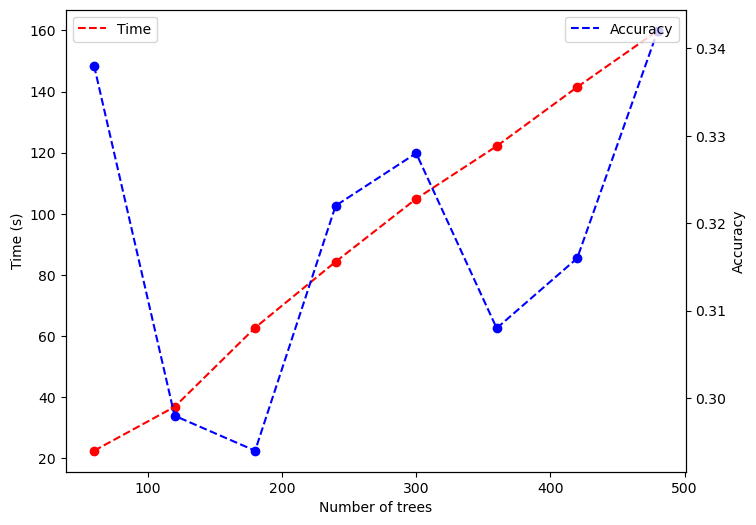
\includegraphics[width=0.7\textwidth,height=0.4\textwidth]{figs/1.png}
    
    \caption{\texttt{n\_estimators}}
    \label{fig:n_estimators}
\end{figure}

\subsubsection{\texttt{max\_depth}}

本实验在CIFAR10数据集上测试, 与实验无关的参数配置如下:

 \begin{lstlisting}[language=bash]
-d cifar10 --n_jobs 50 --n_estimators 50 --min_samples_leaf 1 --min_samples_split 2 
\end{lstlisting}

我们一并测试\texttt{max\_depth}与\texttt{criterion}, 结果如图\ref{fig:max_depth}所示. 

从结果可见, 使用'gini'判别比'entropy'判别需要更长的时间训练模型, 但有更高的准确率. 

模型训练时间随\texttt{max\_depth} 先线性增长, 后几乎不变. 观察决策树深度可知, 这是因为在\texttt{max\_depth}较小时, 它是限制决策树生长的主要因素, 因而训练时间线性增长; 在\texttt{max\_depth}较大时, 它对决策树深度的限制作用减弱, 其他因素如训练样本数的限制作用占主导地位, 因而训练时间几乎不变. 在\texttt{max\_depth}大于25时, 它已经不能限制决策树的深度, 因而不继续增大参数值进行实验.
例如, \texttt{max\_depth}=25,criterion='entropy'时, 所有决策树的深度是: \begin{lstlisting}[language=python]
[21, 18, 20, 20, 19, 20, 20, 25, 24, 21, 17, 18, 19, 19, 24, 17, 18, 20, 17, 21, 19, 25, 21, 21, 21, 20, 19, 24, 24, 19, 18, 19, 18, 21, 21, 20, 19, 20, 21, 19, 18, 18, 18, 18, 17, 18, 17, 18, 19, 21]
\end{lstlisting}

实验中\texttt{max\_depth}与模型准确率的关系不明显,但理论上说, \texttt{max\_depth}较小时, 决策树的分支少, 模型复杂度低, 容易欠拟合; \texttt{max\_depth}较大时, 决策树的分支多, 模型复杂度高. 总的来说, \texttt{max\_depth} 参数起到了模型正则化的作用, 限制决策树的最大深度有避免过拟合,控制训练时间的作用. 

\begin{figure}[h]
    \centering
    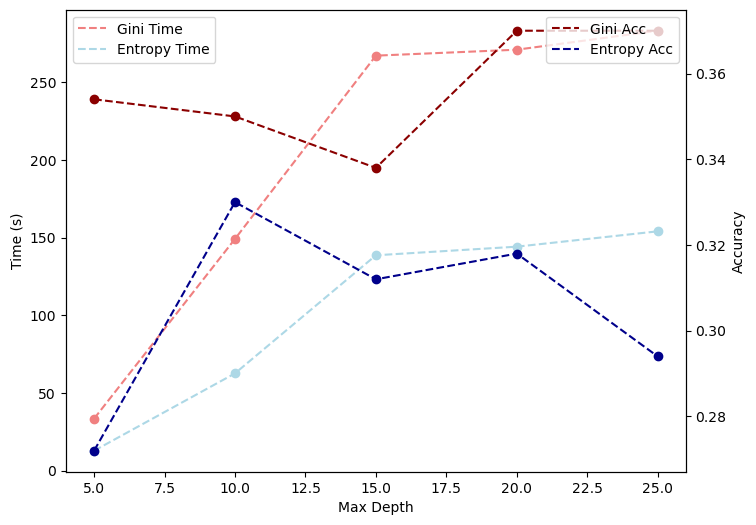
\includegraphics[width=0.7\textwidth,height=0.4\textwidth]{figs/2.png}
    
    \caption{\texttt{max\_depth},\texttt{criterion}}
    \label{fig:max_depth}
\end{figure}

\subsubsection{\texttt{min\_samples\_split},\texttt{min\_samples\_leaf}}
无关参数配置:
 \begin{lstlisting}[language=bash]
-d cifar10 --n_jobs 50 --n_estimators 50 --max_depth 20
\end{lstlisting}

(\texttt{min\_samples\_split},\texttt{min\_samples\_leaf})两个参数同样起到控制叶节点的样本规模的作用,  因而一并实验. 考虑到二者的作用, 这里将他们合称为最小节点样本数.
我们设计以下12组实验, 最小节点样本数逐渐增长: [(1, 2), (2, 5), (3, 6), (2, 10), (3, 10), (5, 30), (10, 20), (10, 50), (20, 40), (10, 100), (20, 100), (20, 300)]. 我们同时测试\texttt{criterion}的影响.

实验结果如图\ref{fig:samples_acc}, 图\ref{fig:samples_time}所示. 其中横坐标是按照上述顺序排列的实验参数的序号.

与先前的结论相同, 'gini'判别比'entropy'判别需要更长的时间训练模型, 但有更高的准确率.

与\texttt{max\_depth}相似, 随着最小节点样本数增加, 模型训练时间单调下降. 使用'gini'判别训练的模型准确率随最小节点样本数增加而下降,  但有一定程度波动. 而使用'entropy'判别训练的模型准确率没有随最小节点样本数明显变化. 后者可能是由于'entropy'判别本身准确率不高, 因而受最小节点样本数的正则化作用影响更小.

总的来说, \texttt{min\_samples\_split}和\texttt{min\_samples\_leaf}同样起到了模型正则化的作用, 可以控制训练时间.
\begin{figure}[h]
    \centering
    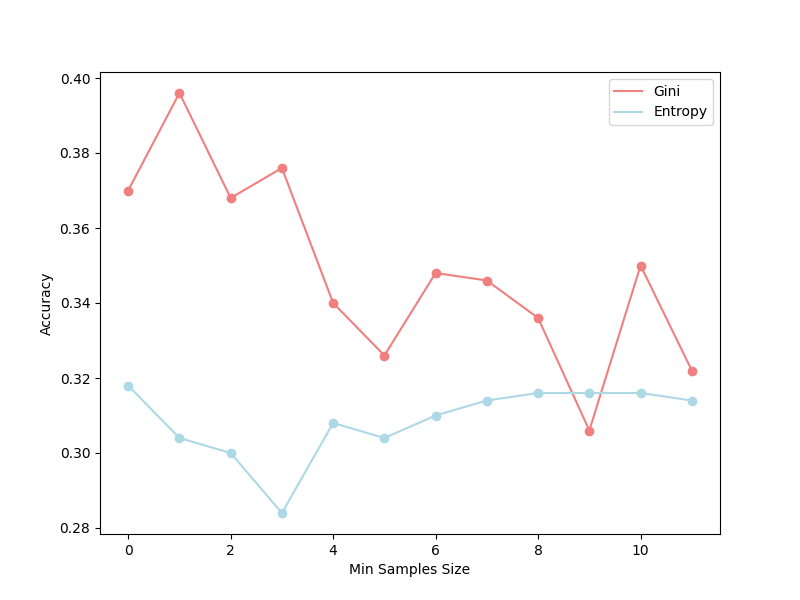
\includegraphics[width=0.7\textwidth,height=0.4\textwidth]{figs/3.png}
    
    \caption{\texttt{min\_samples\_split},\texttt{min\_samples\_leaf}与准确率}
    \label{fig:samples_acc}
\end{figure}

\begin{figure}[h]
    \centering
    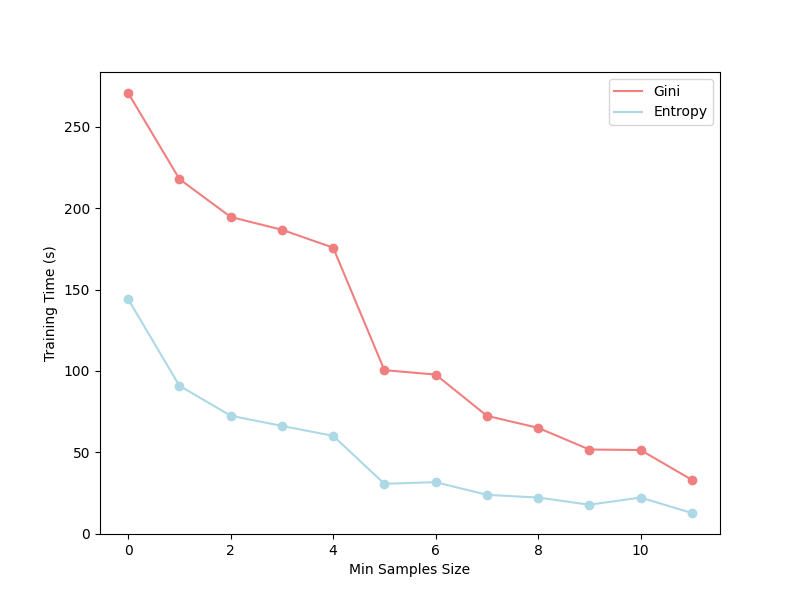
\includegraphics[width=0.7\textwidth,height=0.4\textwidth]{figs/4.png}
    
    \caption{\texttt{min\_samples\_split},\texttt{min\_samples\_leaf}与训练时间}
    \label{fig:samples_time}
\end{figure}

\subsubsection{\texttt{min\_impurity\_decrease}}
无关参数配置:
 \begin{lstlisting}[language=bash]
-d cifar10 --n_jobs 50--n_estimators 50 --max_depth 20 
\end{lstlisting}

\begin{figure}[h]
    \centering
    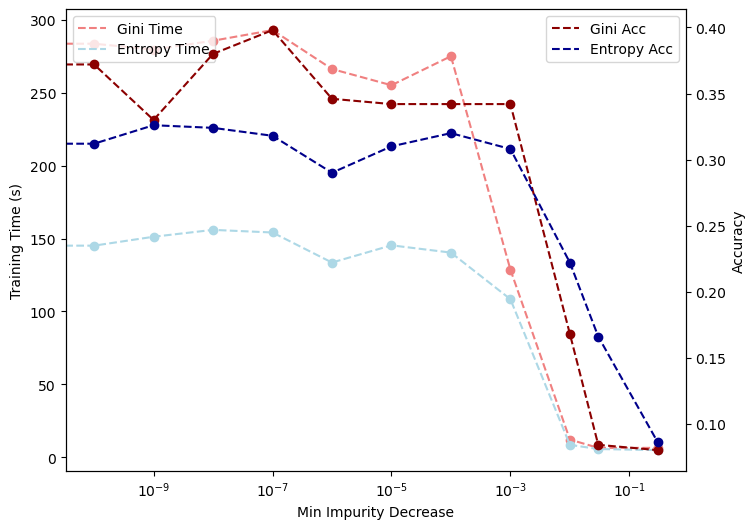
\includegraphics[width=0.7\textwidth,height=0.4\textwidth]{figs/5.png}
    
    \caption{\texttt{min\_impurity\_decrease}}
    \label{fig:mid}
\end{figure}

如图\ref{mid}所示, \texttt{min\_impurity\_decrease}的作用同样是模型正则化. 在参数取值合适时能避免过拟合, 但它在取值偏小时没有明显作用, 在取值偏大时将严重损害模型效果. 

\subsubsection{多类别策略} \label{sec:multiclass}
在随机森林中, 多类别策略主要指软预测与硬预测二者的选取. 我们也可以在每个叶节点使用线性分类器, SVM等其他分类方式, 但这会极大增加模型复杂度, 不完全符合随机森林的设计思想. 这里我们展示在相同参数下在测试集上两种方法的表现. 使用的参数与在\label{sec:best_rf}中相同.

结果如表\ref{table_rf_pred}所示, 可见两种方法的准确率没有明显差异. 二者所用时间有一定差异, 但我们经过重复实验后认为, 这与计算设备的性能波动有关, 没有充分证据认为两种方法的计算性能存在差异.


\begin{table*}[ht]
\centering
\caption{硬预测, 软预测的表现对比}
\begin{tabular}{|c|c|c|c|c|}
\hline
数据集& 预测方法 &准确率&训练时间&测试时间\\
\hline
MNIST & 硬预测&96.0\%  &997.06s & 9.16s\\
MNIST & 软预测 &96.0\%  &595.68s & 5.09s\\
CIFAR10& 硬预测 & 36.8\% &196.94s & 0.46s\\
CIFAR10& 软预测 & 35.9\% &114.94s & 0.36s\\
\hline
\end{tabular}
\label{table_rf_pred}
\end{table*}


\section{多维度节点分类函数}


\subsection{概述}
这部分作业中, 我们主要参考文献\cite{ccf}的方法, 构建Canonical Correlation Forest (CCF)来解决问题, 并通过实验对比了它与随机森林的性能差异.

将节点的分类函数扩展为多维度分类函数有多种思路, 主要思想是将训练数据进行某种线性变换, 再依据变换后的特征进行单维度分类. 具体来说, 进行线性变换可以使用随机旋转, PCA, LDA等方法, 以及下文中将介绍的Canonical Correlation Analysis (CCA)方法.

良好的集成学习泛化性能要求每个基分类器既表现优秀, 又有足够的差异. 仅仅采用随机旋转仅能丰富基分类器的多样性而不能优化其表现. PCA可以将各维度特征变换为正交特征, 但它没有在投影时考虑样本标签, 而且有较高的计算代价, 不适合在每个节点使用. LDA同样可以提升模型性能, 但面临计算效率和数值稳定性的问题. 

CCA\cite{cca}是另一种可用于线性投影的方法. 给定两个行数相同的矩阵$W\in\mathbb {R}^{n\times d}, V\in\mathbb {R}^{n\times k}$, CCA的目标是将它们分别投影到新的空间, 使得二者的相关性最大化. 即寻找一系列的系数对, 使得
$$ {A_1,B_1}= \underset{a\in \mathbb{R}^d,b\in \mathbb{R}^k}{argmax}\   corr(Wa,Vb)$$
满足约束$\| a\|_2=1,\|b\|_2=1$, 对应降维后的Canonical Correlation Components是$WA_1,VB_1$. 用相同的方式可以找到共计$v_{max}=min(rank(W),rank(V))$组系数, 使得各个分量不相关, 即 $\forall i\neq j, (WA_i)^T WA_j=0$  $(VB_i)^T VB_j=0$.

CCA有简单的闭式解和数值稳定的求解算法. 在CCF中, 我们可以将多分类标签以独热编码的形式写成矩阵, 然后以训练样本的多维特征与标签分别为$W,V$求解CCA, 以$WA$作为对多维特征的线性投影. 在新的特征空间按照单维度二分类的方法分类. 

\subsection{Canonical Correlation Forest}

\subsubsection{CCF工作原理}
按照原文献\cite{ccf}的设计, CCF与随机森林的不同之处主要在于:
\begin{enumerate}
    \item 训练时, 在每个节点处选定m个备选特征后, 先对训练样本的特征和标签求解CCA, 再在投影后的特征空间作单维度分类. 在确定分类超平面后, 我们仅需保留对应于分裂特征的一个$A_i$系数, 以供预测时计算.
    \item 不在训练整个基决策树之前进行\texttt{bootstrap}, 而是在计算每个节点的CCA时进行\texttt{projection\_bootstrap}, 即以\texttt{bootstrap}的方式选取部分训练样本来计算投影系数. 在确定分裂超平面时, 仍然使用该节点所有训练样本来计算.
\end{enumerate}
这里不同于原始设计, 我们将\texttt{bootstrap}和\texttt{projection\_bootstrap}视为可调节的参数, 二者的默认值为True.  每个基决策树的完整的训练算法\cite{ccf}如图\ref{fig:train_ccf}.
\begin{figure}[h]
    \centering
    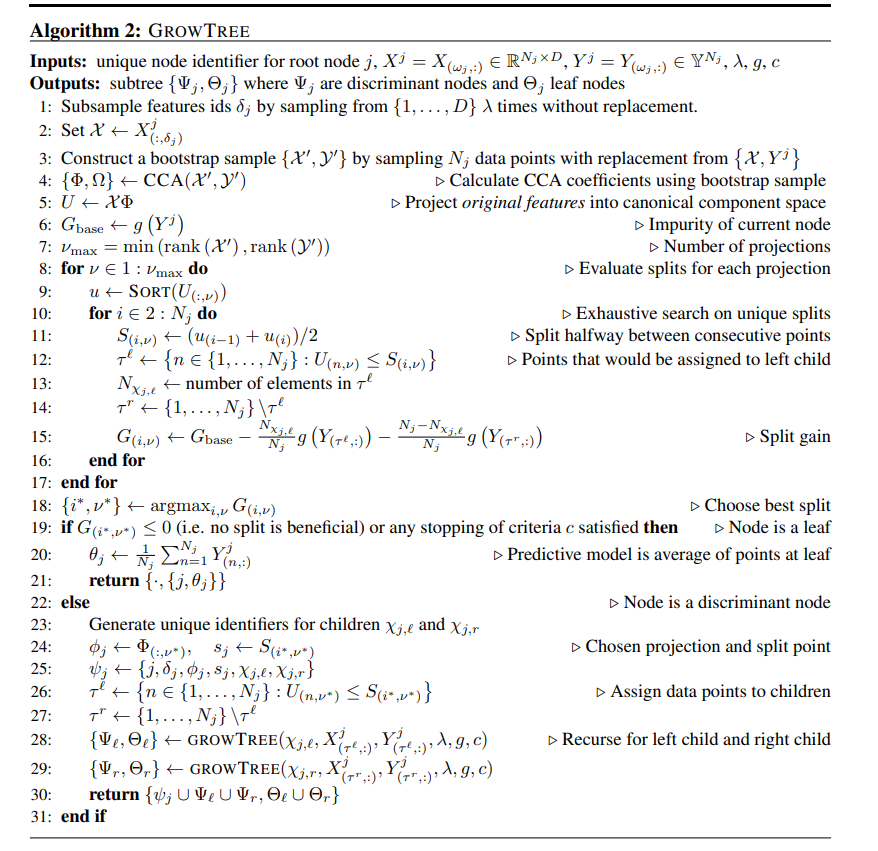
\includegraphics[width=0.7\textwidth,height=0.7\textwidth]{figs/6.png}
    
    \caption{基决策树训练算法}
    \label{fig:train_ccf}
\end{figure}

在随机生成的样例数据集上, CCF的表现如图\ref{fig:dtest_ccf}. 可以看到, 借助CCA进行线性投影可以帮助节点找到合适的决策边界.
\begin{figure}[h]
    \centering
    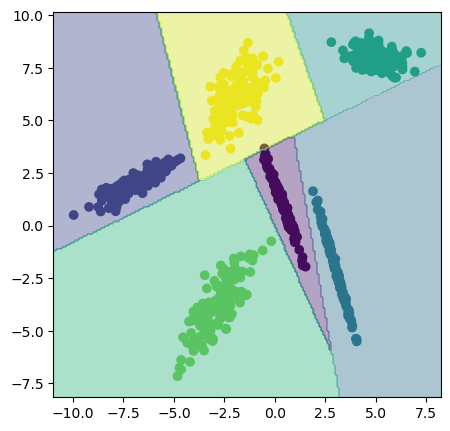
\includegraphics[width=0.35\textwidth,height=0.35\textwidth]{figs/8.png}
    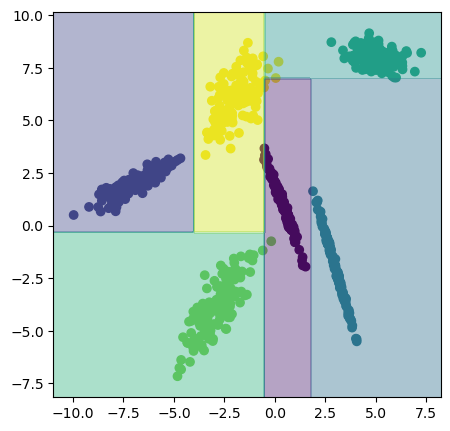
\includegraphics[width=0.35\textwidth,height=0.35\textwidth]{figs/9.png}
    \caption{左为CCF分类效果, 右为随机森林分类效果}
    \label{fig:dtest_ccf}
\end{figure}

\subsubsection{CCA算法实现}
求解CCA的数学推导超出了这份报告的范围, 这里我们仅探讨不同实现的差异.

原文献\cite{ccf}给出了两种CCA的算法实现方式: 简单闭式解法和数值稳定算法. 它声称前者由于需要计算通常非奇异的协方差矩阵的逆, 因而存在数值不稳定的问题. 而如图\ref{fig:cca_nsa}所示的数值稳定算法, 基于QR分解和SVD分解计算, 不存在这个问题. 但原文献的开源代码中CCA的实现仍然使用了闭式解方法. 

我们在\textbf{python}中实现了CCA的数值稳定算法, 并翻译了原文献的算法实现. 经过实际测试, 我们发现直接运行上述数值稳定算法是极低效的. 具体来说, 它需要在决策树的每个节点都计算矩阵$W,V$的QR分解, 这是不可接受的. 例如在MNIST数据集中, (在划分$10\%$的验证集后)训练样本特征的维度是$[54000,784]$, 则Q,R矩阵的维度分别是$[54000,54000],[54000,784]$, 此时Q矩阵共有$2.916*10^{9}$个元素, 若以32位浮点数存储, 需要占用约11GB内存. 而原文献的方法有更好的计算效率和内存占用,  因而我们在后续过程中使用这种方法计算CCA.

\begin{figure}[h]
    \centering
    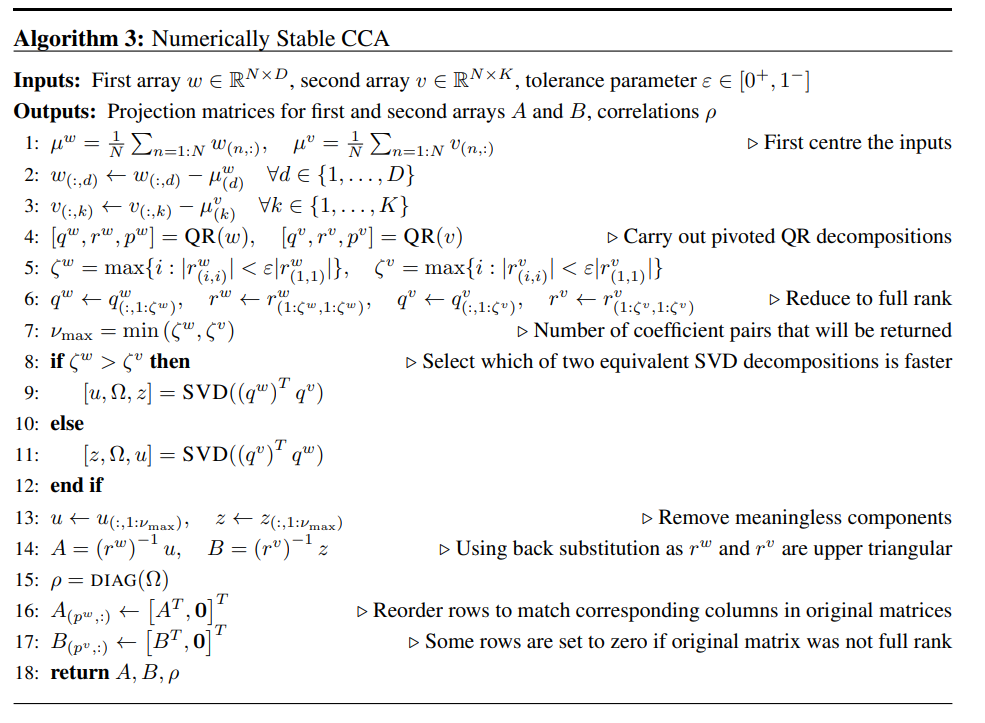
\includegraphics[width=0.7\textwidth,height=0.5\textwidth]{figs/7.png}
    
    \caption{CCA的数值稳定算法}
    \label{fig:cca_nsa}
\end{figure}

\subsection{最佳表现}
我们选取最优参数后, 得到测试集上的结果如表\ref{table_ccf_perf}. 总的来说, CCF算法的准确率与RF相近. 添加CCA处理没有增加训练时间, 这可能是因为使用CCA处理后, 每个节点的分类能力增强 每个决策树需要构建的节点数量减少, 因而训练时间没有增加(请参考\ref{sec:multiclass}中关于RF结果的补充分析).

\begin{table*}[ht]
\centering
\caption{MNIST和CIFAR10数据集上CCF的最佳表现}
\begin{tabular}{|c|c|c|c|c|c|}
\hline
数据集& RF准确率 &CCF准确率&训练时间&测试时间\\
\hline
MNIST & 96.0\% & 95.3\%  &462.58s & 6.02s\\
CIFAR10& 36.8\% & 36.8\% &53.02s & 1.38s\\
\hline
\end{tabular}
\label{table_ccf_perf}
\end{table*}


在MNIST数据集上使用的配置是:
 \begin{lstlisting}[language=bash]
-d mnist --rf_type ccf --n_jobs 30 --criterion gini --n_estimators 60 --max_depth 20 --min_samples_split 20 --min_samples_leaf 2  --min_impurity_decrease 1e-12
\end{lstlisting}

 在CIFAR10数据集上使用的配置是:
 \begin{lstlisting}[language=bash]
-d cifar10 --rf_type ccf --n_jobs 20 --criterion entropy --soft_pred --n_estimators 65 --max_depth 27 --min_samples_split 2 --min_samples_leaf 56 --min_impurity_decrease 2.07e-14
\end{lstlisting}

\subsection{参数消融实验}
% \subsubsection{重复先前的测试项}
与RF相同, 我们在验证集上进行实验. 因为这部分的结论和分析与\ref{sec:rf_exp}中相同, 我们仅放出实验结果, 不重复分析. 关于\texttt{criterion},  \texttt{n\_estimators}, \texttt{max\_depth}, \texttt{min\_samples\_split}, \texttt{min\_samples\_leaf}, \texttt{min\_impurity\_decrease}的实验结果如图\ref{fig:ccf_exp1}. 

另外, 关于\texttt{soft\_pred},\texttt{bootstrap},\texttt{projection\_bootstrap}的实验如下表\ref{table_ccf_exp}. 可见这3个选项对训练和测试时间几乎没有影响.\texttt{projection\_bootstrap}=False会降低模型准确率, 其他参数对准确率的影响不明显. 这一组实验的默认配置如下:
 \begin{lstlisting}[language=bash]
-d cifar10 --rf_type ccf --n_jobs 30 --criterion entropy --soft_pred --n_estimators 65 --max_depth 27 --min_samples_split 2 --min_samples_leaf 56 --min_impurity_decrease 2.07e-14
\end{lstlisting}

\begin{figure}[h]
    \centering
    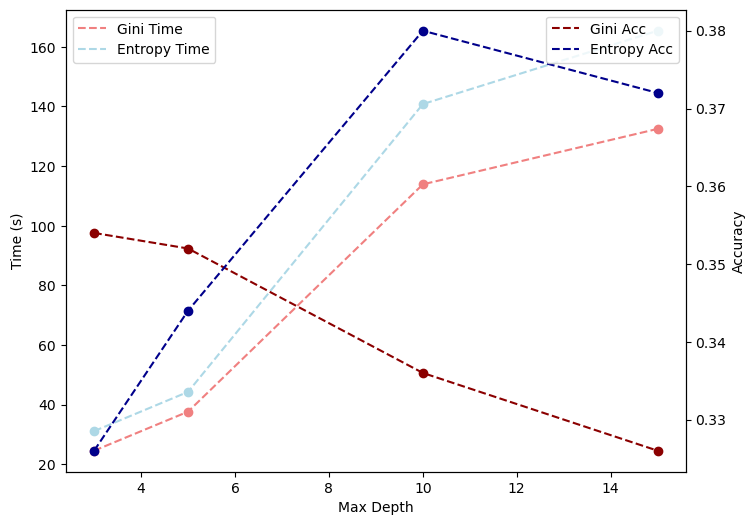
\includegraphics[width=0.45\textwidth,height=0.3\textwidth]{figs/11.png}
    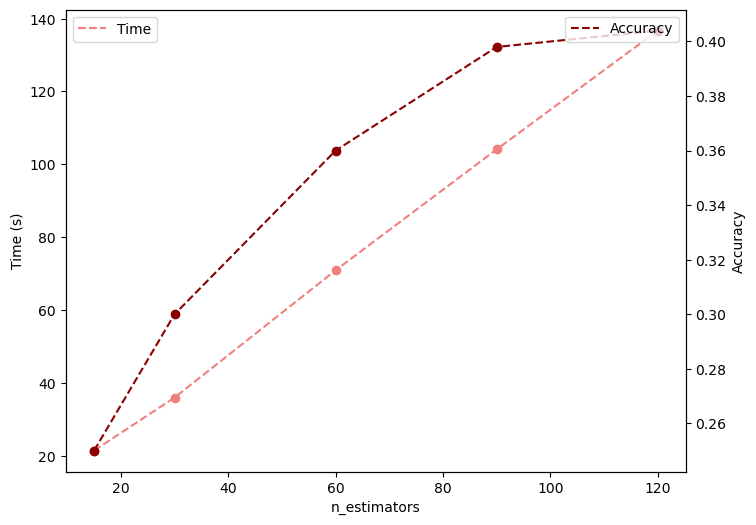
\includegraphics[width=0.45\textwidth,height=0.3\textwidth]{figs/12.png}
    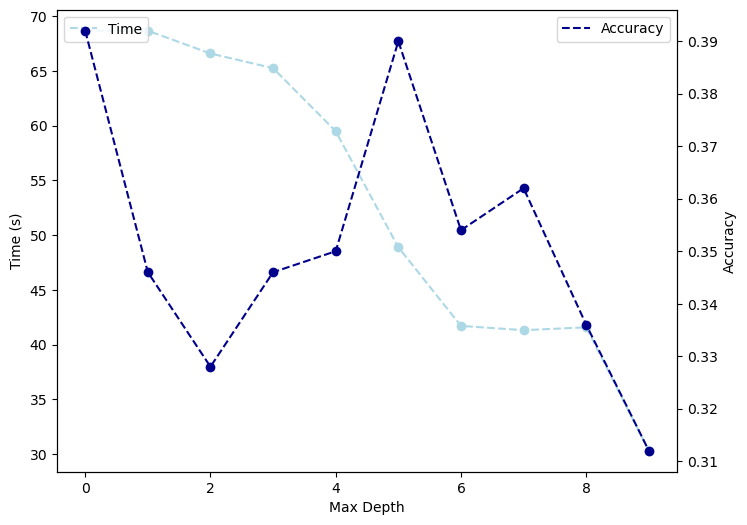
\includegraphics[width=0.45\textwidth,height=0.3\textwidth]{figs/13.png}
    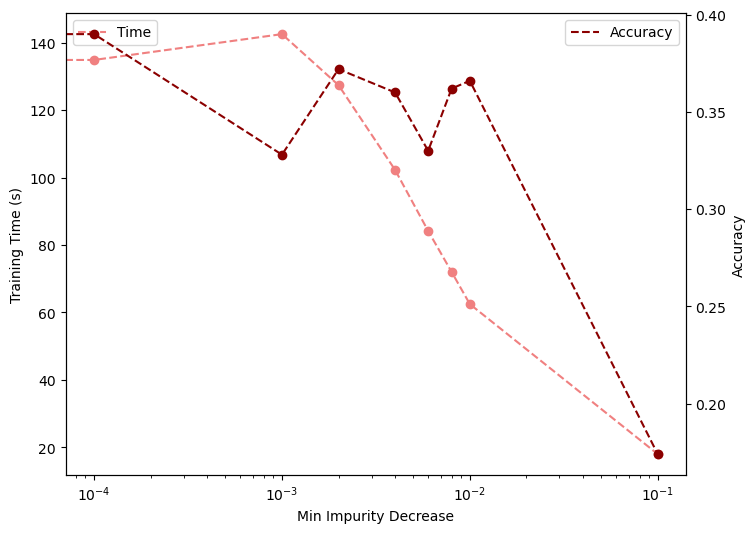
\includegraphics[width=0.45\textwidth,height=0.3\textwidth]{figs/14.png}
    
    \caption{CCF上的参数消融实验}
    \label{fig:ccf_exp1}
\end{figure}

\begin{table*}[ht]
\centering
\caption{CCF对比实验}
\begin{tabular}{|c|c|c|c|c|c|}
\hline
实验&准确率&训练时间&测试时间\\
\hline
默认 &36.4\%  &56.26s & 1.45s\\
\texttt{soft\_pred}=False & 36.8\% &56.24s & 1.46s\\
\texttt{bootstrap}=False & 36.1\% &54.37s & 1.43s\\
\texttt{projection\_bootstrap}=False & 35.0\% &55.38s & 1.45s\\
\hline
\end{tabular}
\label{table_ccf_exp}
\end{table*}

\section{总结}

这次作业中, 我们从零开始实现了随机森林分类器, 并基于此实现了CCF分类器. 这两个算法在MNIST数据集上分别达到了$96.0\%$, $95.3\%$的分类准确率, 而在CIFAR10数据集上均达到了$36.8\%$的准确率, 这与\texttt{sklearn}库的随机森林分类器相近. 

此外我们通过消融实验探究了不同参数对这两个模型表现的影响. 基决策树的个数决定模型的效果, 模型训练时间随着它线性增长; 在它的值较小时, 增大它能有效提升模型的性能, 捕捉数据的规律, 但当它达到一定程度后, 增大它仅能降低模型方差, 难以提高模型泛化性.基决策树的最大深度, 最小分裂样本数, 最小节点样本数, 最小不纯度下降这4个参数都控制着决策树的规模, 它们通过控制节点的分裂与否, 起到正则化和控制训练时间的作用. 模型的多分类策略有硬预测与软预测两种 在CCF中, 使用自举与投影自举都是增大基决策树随机性的方式.

CCF分类器有较为优秀的设计, 它通过在每个节点计算CCA将输入特征和标签投影到相关性最高的空间, 这有利于对投影后的特征进行单维度二分类, 直觉上能提高每个节点的分类增益. 但在实验中它没有明显优于随机森林分类器, 甚至性能有所下降, 可能是由于数据集本身的规律所限. 本质上说, 随机森林与CCF分类器都是线性分类器的反复叠加. 对于规律复杂, 严重非线性, 特征各维度高度相关的数据分布, 这两种分类器的准确率相近是非常合理的. 使用SIFT, 边缘检测等方式进行图像特征提取可能有助于进一步提升模型性能.

受限于时间, 数学水平, 计算资源等因素, 我们的实验有许多缺陷. 尽管CCA的数学特性令人影响深刻,但由于线性代数等相关知识的不足, 我们没能深入透彻地理解CCA及其算法实现. 在我们的实验中没能进行重复对比试验, 计算平均值, 标准差等统计量, 结果中许多参数的不同选择之间的差异不显著, 不能得出有说服力的推论. 我们的算法实现仍有较大的优化的空间, 相比于\texttt{sklearn}库提供的分类器, 我们的计算效率低下, 存在约$10\sim 20$倍的性能差距.

\section{致谢}
感谢倪冰冰老师及机器学习课程助教.

感谢张睿, 李天骅等与我讨论交流的同学.

\begin{thebibliography}{99}  

\bibitem{ccf}Rainforth, T., and Wood, F. (2015): Canonical correlation forest, arXiv preprint, arXiv:1507.05444.
\bibitem{cca}Harold Hotelling. Relations between two sets of variates. Biometrika, pages 321–377, 1936.
\bibitem{cca_zhihu}Canonical Correlation Analysis - 知乎:\href{https://zhuanlan.zhihu.com/p/52717082}{https://zhuanlan.zhihu.com/p/52717082}
\bibitem{sklearn}sklearn.ensemble.RandomForestClassifier:

\href{ https://scikit-learn.org/stable/modules/generated/sklearn.ensemble.RandomForestClassifier.html#sklearn.ensemble.RandomForestClassifier}{https://scikit-learn.org/stable/modules/generated/sklearn.ensemble.RandomForestClassifier.html}
\end{thebibliography}
\end{document}